% =====================================================================
% Supplementary results appendix. Paste after \appendix and BEFORE the
% AI/LLM disclosure section (or keep this file and use % =====================================================================
% Supplementary results appendix. Paste after \appendix and BEFORE the
% AI/LLM disclosure section (or keep this file and use % =====================================================================
% Supplementary results appendix. Paste after \appendix and BEFORE the
% AI/LLM disclosure section (or keep this file and use % =====================================================================
% Supplementary results appendix. Paste after \appendix and BEFORE the
% AI/LLM disclosure section (or keep this file and use \input{appendix_results}).
% Needs: booktabs, multirow, graphicx (already loaded in main.tex).
% Figures: upload report/figures/*.pdf to the Overleaf "figures/" folder.
% Annotators are A1--A4, consistent with Table 1 in the main text.
% =====================================================================

\section{Supplementary Results}
\label{app:results}

This appendix reports results and implementation details that support the main
text but did not fit in the page limit. All numbers are regenerated by the
scripts in the repository (\texttt{src/analysis\_\{a,b,c\}/analyze.py},
\texttt{src/analysis\_c/predict.py}).

% ---------------------------------------------------------------------
\subsection{Implementation details}
\label{app:impl}

\paragraph{Subset.} 90 items sampled with seed 42, 30 per audio type. Item 1091
is excluded because two of its options are identical, which makes its correct
letter ambiguous. All three analyses use this subset; Analysis~1 uses 50 of the
90 items.

\paragraph{Model and prompt.} We use the text-output component (``thinker'') of
Qwen2.5-Omni-3B in bfloat16 with the default Qwen system prompt, on an Apple M2
Max (PyTorch 2.14.1 with the MPS backend, \texttt{transformers} 5.18.0). The user
turn contains the raw media (if any), then the surrogate lines
\texttt{Image description:~\ldots} and/or \texttt{Audio transcript/description:~\ldots}
(if any), then \texttt{Question:~\ldots}, the options \texttt{A.}--\texttt{D.}, and
the instruction \emph{``Answer with the option's letter from the given choices
directly.''} Images are resized with Qwen's own resizing to at most
$768\times28\times28$ pixels (at most 768 visual tokens; mean 700). Audio is
resampled to 16\,kHz mono and costs 25 tokens per second (mean 270 tokens).

\paragraph{Scoring.} One forward pass per input. We take the next-token logits
at the answer position, keep the four letter tokens (each A--D is a single
token), and apply a softmax. In a 55-pass check, the highest-scoring vocabulary
token was always one of the four letters, and greedy generation always began
with the argmax letter. For shuffled orders, probabilities are mapped back to the
original options before scoring correctness.

\paragraph{Option orders.} Order 0 is the original; orders 1 and 2 are random
permutations seeded by (seed, item, order) and redrawn until they differ from the
earlier orders. Every configuration is run under all three orders (1,890 forward
passes in total).

\paragraph{Cost measurements.} Input tokens are counted by modality directly
from the processed input ids; ``text'' tokens include the system prompt and chat
template (about 110 tokens per item). Latency covers the forward pass only, with
batch size 1, three warm-up passes, and device synchronization before and after.
PyTorch's MPS backend has no peak-memory counter, so a background thread samples
allocated memory every 2\,ms during each pass; we report the peak minus the
pre-pass baseline (activation memory), which is approximate. Model weights take
about 9.05\,GB.

% ---------------------------------------------------------------------
\subsection{Analysis 1: additional human results}
\label{app:a1}

\begin{table}[h]
\caption{Pairwise agreement on the 10 shared items (Cohen's $\kappa$).}
\label{tab:app-pairs}
\centering\small
\begin{tabular}{lcccc}
\toprule
 & \multicolumn{2}{c}{Final answer} & \multicolumn{2}{c}{``Text is enough''} \\
Pair & Agree & $\kappa$ & Agree & $\kappa$ \\
\midrule
A1--A2 & 40\% & 0.22 & 70\% & 0.44 \\
A1--A3 & 50\% & 0.35 & 60\% & 0.17 \\
A1--A4 & 40\% & 0.20 & 80\% & 0.55 \\
A2--A3 & 50\% & 0.32 & 30\% & $-0.30$ \\
A2--A4 & 40\% & 0.24 & 50\% & 0.19 \\
A3--A4 & 30\% & 0.05 & 40\% & $-0.36$ \\
\midrule
All four (Fleiss) & -- & 0.22 & -- & 0.08 \\
\bottomrule
\end{tabular}
\end{table}

\begin{table}[h]
\caption{The 10 shared items: how many of the four annotators answered correctly, how many distinct
final answers they gave, and how many judged the text sufficient.}
\label{tab:app-shared}
\centering\small
\setlength{\tabcolsep}{4pt}
\begin{tabular}{rllcccc}
\toprule
Item & Audio & Task & Gold & Correct & Distinct & Text enough \\
\midrule
66   & speech & Action      & D & 0/4 & 3 & 3/4 \\
323  & speech & Plot        & D & 1/4 & 3 & 3/4 \\
389  & speech & Plot        & A & 0/4 & 2 & 1/4 \\
641  & speech & Context     & C & 3/4 & 2 & 1/4 \\
745  & sound  & Action      & C & 1/4 & 2 & 3/4 \\
847  & sound  & Story       & D & 3/4 & 2 & 1/4 \\
1019 & sound  & Action      & C & 2/4 & 3 & 1/4 \\
1057 & music  & Object ID   & C & 1/4 & 3 & 3/4 \\
1070 & music  & Story       & B & 4/4 & 1 & 4/4 \\
1086 & music  & Action      & B & 0/4 & 2 & 3/4 \\
\bottomrule
\end{tabular}
\end{table}

\paragraph{Agreement.} \Cref{tab:app-pairs,tab:app-shared} break down the low
agreement reported in \cref{sec:a1}. Agreement on the final answer is uniformly
low (30--50\% per pair), and agreement on ``text is enough'' is inconsistent:
some pairs agree reasonably (A1--A4, $\kappa{=}0.55$) while others disagree more
than chance would predict (A3--A4, $\kappa{=}-0.36$). Three shared items were
answered correctly by nobody, and on two of them most annotators had judged the
text sufficient, which illustrates the overconfidence in \cref{tab:annotators}.
Only item 1070 was answered correctly and unanimously.

\begin{table}[h]
\caption{Human results by audio type and task type (80 annotations). \emph{Text}: accuracy of stage-0
text-only answers; \emph{Final}: after revealing.}
\label{tab:app-human-breakdown}
\centering\small
\setlength{\tabcolsep}{4pt}
\begin{tabular}{lcccc}
\toprule
 & $n$ & Said enough & Text & Final \\
\midrule
Speech      & 29 & 62\% & 38\% & 41\% \\
Sound event & 26 & 62\% & 32\% & 54\% \\
Music       & 25 & 64\% & 45\% & 40\% \\
\midrule
Action and Activity          & 30 & 60\% & 19\% & 40\% \\
Plot Inference               & 18 & 61\% & 50\% & 44\% \\
Story Description            & 14 & 57\% & 50\% & 57\% \\
Contextual / Environmental   &  9 & 56\% & 44\% & 56\% \\
Object Identification        &  9 & 89\% & 44\% & 33\% \\
\bottomrule
\end{tabular}
\end{table}

\paragraph{By audio and task type.} \Cref{tab:app-human-breakdown} is in line
with H1.2: revealing the raw inputs helped most for sound events (32\% $\to$
54\%), whose transcripts are short descriptions, and for action questions
(19\% $\to$ 40\%). It did not help for music (45\% $\to$ 40\%). Annotators judged
text sufficient at similar rates for every audio type (62--64\%), even though
text-only accuracy differed. With 9--30 annotations per row, these breakdowns are
descriptive only.

\paragraph{Reveal behavior and cost.} Annotators revealed both modalities in 79
of 80 items and revealed the image first in 78. As a result, the token cost of
their information use (computed from each item's per-modality token counts in
Analysis~2) was uninformative: the mean was 1.26$\times$ the full-input cost,
since they read the caption and transcript as well as viewing both raw inputs.
Free-text notes named the audio as decisive in 33 annotations, the image in 31,
and the text in 26 (multiple labels allowed).

% ---------------------------------------------------------------------
\subsection{Analysis 2: additional model results}
\label{app:a2}

\begin{figure}[h]
\centering
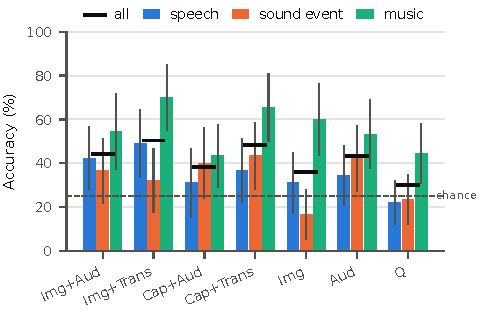
\includegraphics[width=\columnwidth]{figures/acc_by_config_audio.pdf}
\caption{Accuracy by input configuration and audio type (mean over three option orders), with 95\%
confidence intervals over items. Black ticks show the accuracy over all 90 items.}
\label{fig:app-acc-bars}
\end{figure}

\begin{table*}[t]
\caption{Full per-configuration results. Accuracy is shown both in the original option order and
averaged over three orders. Token counts and latency are means per item; \emph{Act.\ mem.} is the
activation memory (approximate on MPS); \emph{Max prob} is the mean probability of the predicted option.}
\label{tab:app-config}
\centering\small
\resizebox{\textwidth}{!}{%
\begin{tabular}{lccccccccc}
\toprule
Input & Acc.\ (orig.) & Acc.\ (avg.) & Image tok. & Audio tok. & Text tok. & Lat.\ mean (s) & Lat.\ p90 (s) & Act.\ mem.\ (MB) & Max prob \\
\midrule
Image+Audio        & 38.9 & 44.4 & 700 & 270 & 136 & 3.31 & 4.01 & 327 & .71 \\
Image+Transcript   & 47.8 & 50.4 & 700 &   0 & 161 & 2.66 & 3.00 & 255 & .76 \\
Caption+Audio      & 40.0 & 38.1 &   0 & 270 & 401 & 1.39 & 2.37 & 197 & .70 \\
Caption+Transcript & 46.7 & 48.5 &   0 &   0 & 427 & 0.77 & 0.95 & 126 & .72 \\
Image only         & 33.3 & 35.9 & 700 &   0 & 134 & 2.62 & 2.92 & 246 & .74 \\
Audio only         & 40.0 & 43.3 &   0 & 270 & 134 & 0.98 & 1.84 & 119 & .66 \\
Question only      & 30.0 & 30.0 &   0 &   0 & 132 & 0.31 & 0.39 &  39 & .52 \\
\bottomrule
\end{tabular}}
\end{table*}

\paragraph{Costs.} \Cref{tab:app-config} gives the full cost breakdown. Latency
and activation memory follow the token count closely, except that image tokens
are more expensive per token than text or audio tokens: image-only (834 tokens)
takes 2.6\,s, while caption+audio (671 tokens) takes 1.4\,s. This is because the
vision encoder runs on about four times as many patches before merging. A caption
costs 268 tokens on average but is much longer for music items, so on music the
cost advantage of caption+transcript shrinks.

\begin{table}[h]
\caption{Robustness to option order: accuracy in each order, the share of items answered correctly in
all three orders, and the share where the model gives the same answer in all three.}
\label{tab:app-perm}
\centering\small
\setlength{\tabcolsep}{3.5pt}
\begin{tabular}{lccccc}
\toprule
Input & Ord.\ 0 & Ord.\ 1 & Ord.\ 2 & All correct & Same answer \\
\midrule
Image+Audio        & 38.9 & 48.9 & 45.6 & 33.3 & 65.6 \\
Image+Transcript   & 47.8 & 54.4 & 48.9 & 40.0 & 71.1 \\
Caption+Audio      & 40.0 & 36.7 & 37.8 & 26.7 & 63.3 \\
Caption+Transcript & 46.7 & 48.9 & 50.0 & 35.6 & 62.2 \\
Image only         & 33.3 & 38.9 & 35.6 & 25.6 & 67.8 \\
Audio only         & 40.0 & 45.6 & 44.4 & 27.8 & 57.8 \\
Question only      & 30.0 & 33.3 & 26.7 & 11.1 & 33.3 \\
\bottomrule
\end{tabular}
\end{table}

\begin{table}[h]
\caption{Share of the model's predicted letters (\%, all orders) per configuration, vs.\ the share of
gold answers at each position in the original order.}
\label{tab:app-letters}
\centering\small
\begin{tabular}{lcccc}
\toprule
 & A & B & C & D \\
\midrule
Gold (original order, subset) & 8 & 27 & 22 & 43 \\
\midrule
Image+Audio        & 24 & 34 & 23 & 20 \\
Image+Transcript   & 27 & 32 & 21 & 20 \\
Caption+Audio      & 21 & 43 & 20 & 16 \\
Caption+Transcript & 21 & 44 & 17 & 19 \\
Image only         & 24 & 35 & 23 & 18 \\
Audio only         & 23 & 39 & 23 & 16 \\
Question only      & 23 & 49 & 19 &  9 \\
\bottomrule
\end{tabular}
\end{table}

\paragraph{Option-order effects.} \Cref{tab:app-perm} shows that accuracy can
move by up to 10 points between orders for the same configuration (Image+Audio:
38.9\% to 48.9\%), and that the model gives the same answer in all three orders
on only 58--71\% of items, or 33\% for question only, which is essentially guessing.
\Cref{tab:app-letters} shows the source: the model over-predicts ``B'' in every
configuration, most strongly when it has the least information (49\% for question
only), while the gold answers are concentrated at ``D''.

\begin{figure}[h]
\centering
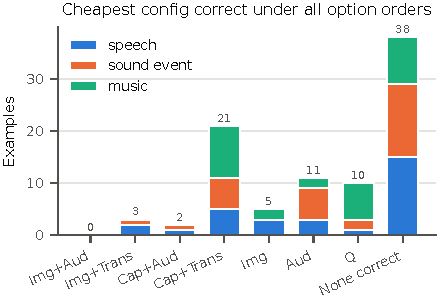
\includegraphics[width=\columnwidth]{figures/oracle_routing.pdf}
\caption{For each item, the cheapest configuration that is correct under all three option orders
(the permutation-robust oracle), stacked by audio type.}
\label{fig:app-oracle}
\end{figure}

\paragraph{Oracle routing.} \Cref{fig:app-oracle} shows which configuration the
permutation-robust oracle picks. Caption+transcript is the cheapest robust
solution for 21 items (10 of them music), audio only for 11 (6 sound events), and
question only for 10 (7 music). The full input is never the cheapest robust
solution, and 38 items (15 speech, 14 sound, 9 music) are not solved robustly by
any configuration. The oracle reaches 57.8\% accuracy at 25\% of the full-input
cost, whereas an oracle over the original order alone reports 68.9\% at 22\%,
inflated by lucky guesses.

\begin{figure}[h]
\centering
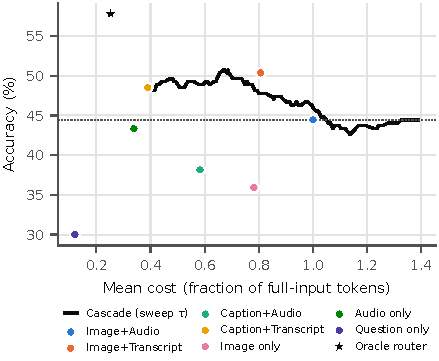
\includegraphics[width=\columnwidth]{figures/cascade.pdf}
\caption{Confidence cascade: answer from caption+transcript and escalate to the full input when the
maximum option probability is below $\tau$ (curve traced by sweeping $\tau$; accuracy averaged over
option orders). Points are the fixed configurations; the star is the permutation-robust oracle.}
\label{fig:app-cascade}
\end{figure}

\paragraph{Cascade.} \Cref{fig:app-cascade} traces the cascade as the threshold
$\tau$ varies. Escalating a few low-confidence items raises accuracy slightly
(peak 50.7\% at 67\% of the cost, $\tau{=}0.565$, escalating 28\% of items), but
escalating more lowers it toward the full-input level (44.4\%), because the full
input is not more accurate than caption+transcript. The cascade never reaches the
oracle; this gap is the headroom a learned router would need to close.

\begin{figure}[h]
\centering
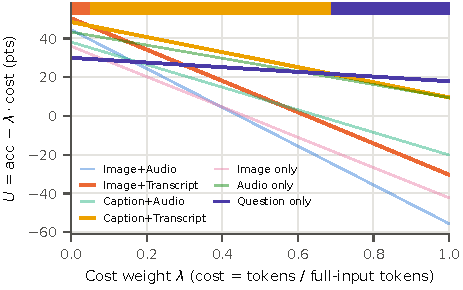
\includegraphics[width=\columnwidth]{figures/utility_sweep.pdf}
\caption{Utility $U{=}\text{acc}-\lambda\cdot\text{cost}$ per configuration as the cost weight $\lambda$
varies; the colored strip at the top marks the optimal configuration.}
\label{fig:app-utility}
\end{figure}

\paragraph{Utility sweep.} \Cref{fig:app-utility} shows which configuration is
optimal as cost is weighted more heavily. Image+transcript is optimal only when
cost barely matters ($\lambda\le0.04$), caption+transcript for
$0.05\le\lambda\le0.68$, and question only beyond that. A single fixed choice is
therefore near-optimal for most cost preferences, so a router's gains must come
from per-item decisions rather than from choosing a better global configuration.

% ---------------------------------------------------------------------
\subsection{Analysis 3: additional language results}
\label{app:a3}

\begin{figure*}[t]
\centering
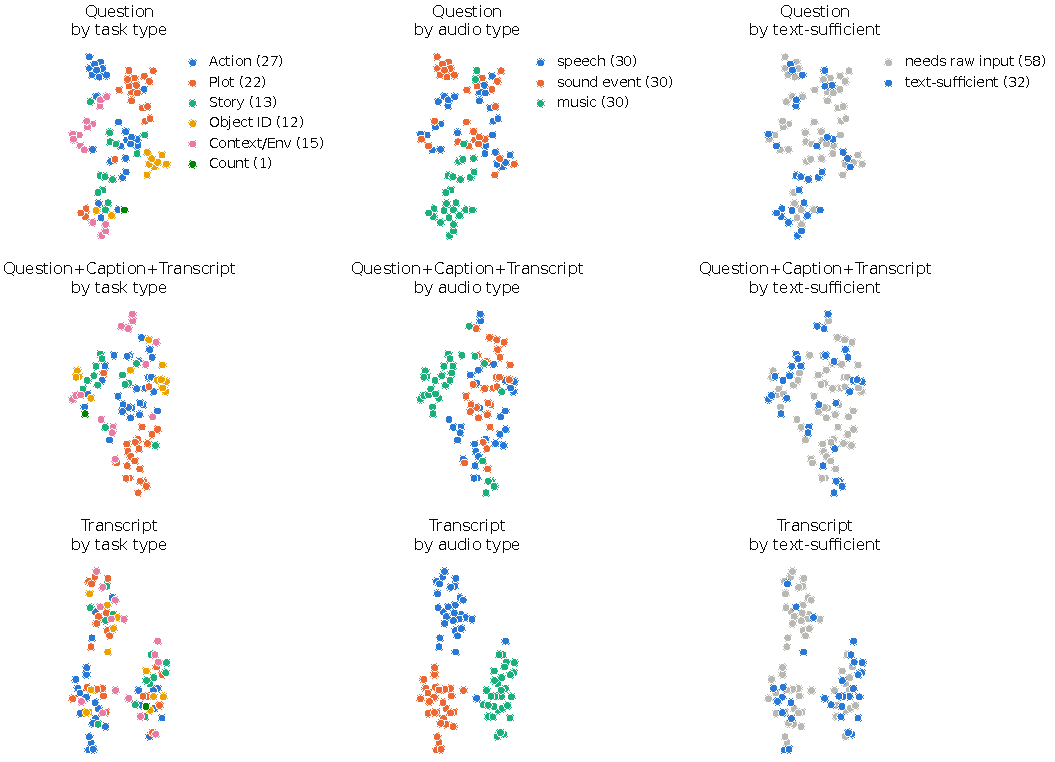
\includegraphics[width=\textwidth]{figures/tsne_grid.pdf}
\caption{t-SNE of SBERT embeddings for the three text views (rows), colored by task type, audio type,
and the model's text-sufficient label (columns). Counts are given in the legends.}
\label{fig:app-tsne-grid}
\end{figure*}

\begin{table}[h]
\caption{Cosine silhouette scores of each grouping in each embedding view (higher means the
grouping is more separated; about 0 means no separation).}
\label{tab:app-sil}
\centering\small
\setlength{\tabcolsep}{4pt}
\begin{tabular}{lcccc}
\toprule
View & Task & Audio & Text-suff.\ (model) & Text-suff.\ (human) \\
\midrule
Question                    & 0.12 & 0.06 & 0.01 & $-0.01$ \\
Question+Caption+Transcript & 0.04 & 0.07 & 0.01 & $-0.02$ \\
Transcript                  & $-0.09$ & 0.19 & 0.01 & $-0.01$ \\
\bottomrule
\end{tabular}
\end{table}

\paragraph{Embedding structure.} \Cref{fig:app-tsne-grid,tab:app-sil} extend
\cref{fig:tsne} to all three views. Question embeddings group mostly by task type
(e.g.\ ``what will happen next'' questions cluster together), transcript embeddings
by audio type, and the combined view shows weak structure for both. No view
separates text-sufficient items, under either model or human labels.

\begin{figure}[h]
\centering
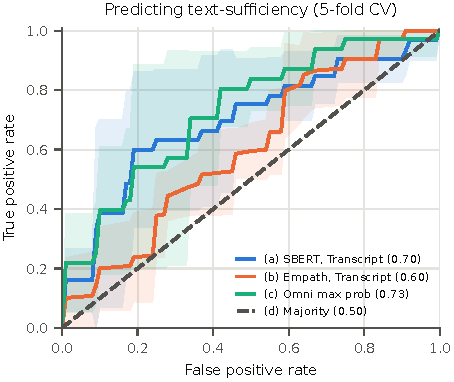
\includegraphics[width=\columnwidth]{figures/predict_roc.pdf}
\caption{Mean ROC curves over five folds (bands: $\pm$1 std) for the best view of each predictor
(model labels). AUROC in parentheses.}
\label{fig:app-roc}
\end{figure}

\begin{figure}[h]
\centering
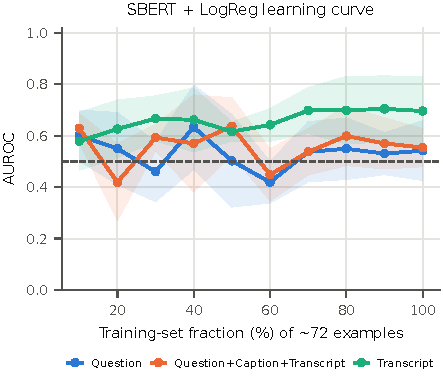
\includegraphics[width=\columnwidth]{figures/predict_learning_curve.pdf}
\caption{Learning curve of SBERT + logistic regression: AUROC on held-out folds when training on a
fraction of each training split (bands: $\pm$1 std over folds; model labels).}
\label{fig:app-lc}
\end{figure}

\paragraph{ROC and learning curves.} In \cref{fig:app-roc}, the model's
confidence and the transcript embeddings perform similarly at low false-positive
rates, and the confidence is better at moderate rates (0.35--0.7); Empath stays
close to chance below a false-positive rate of 0.25. Unlike the transcript
predictor, the confidence needs no training. In \cref{fig:app-lc}, only
the transcript view improves with more data (0.58 at 10\% to 0.70 at 100\%); the
question view stays near chance (0.60 to 0.54) and the combined view does not
improve (0.63 to 0.55). More data might help a transcript-based predictor
somewhat, but it would mostly learn the audio type.

\begin{figure}[h]
\centering
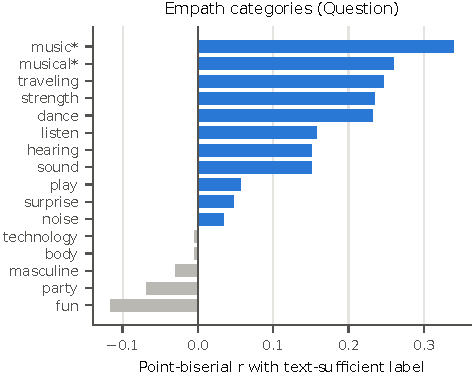
\includegraphics[width=\columnwidth]{figures/empath_top_question.pdf}
\caption{Empath categories in the question text most associated with the model's text-sufficient label
(point-biserial $r$). * marks Benjamini--Hochberg $q<0.05$ over 194 categories.}
\label{fig:app-empath}
\end{figure}

\paragraph{Empath.} \Cref{fig:app-empath} shows the strongest question-view
associations. Only \emph{music} and \emph{musical} survive correction, and the
next categories (\emph{dance}, \emph{listen}, \emph{hearing}, \emph{sound}) are also
audio-related. In the combined view the top categories (\emph{love}, \emph{fire},
\emph{beauty}; $r\approx0.27$--$0.30$) do not survive correction ($q\ge0.35$).
With human labels, nothing survives in any view (smallest $q{=}0.31$). The
interpretable features therefore recover the same signal as the embeddings,
namely the audio type, rather than identifying content that is answerable from
text.
).
% Needs: booktabs, multirow, graphicx (already loaded in main.tex).
% Figures: upload report/figures/*.pdf to the Overleaf "figures/" folder.
% Annotators are A1--A4, consistent with Table 1 in the main text.
% =====================================================================

\section{Supplementary Results}
\label{app:results}

This appendix reports results and implementation details that support the main
text but did not fit in the page limit. All numbers are regenerated by the
scripts in the repository (\texttt{src/analysis\_\{a,b,c\}/analyze.py},
\texttt{src/analysis\_c/predict.py}).

% ---------------------------------------------------------------------
\subsection{Implementation details}
\label{app:impl}

\paragraph{Subset.} 90 items sampled with seed 42, 30 per audio type. Item 1091
is excluded because two of its options are identical, which makes its correct
letter ambiguous. All three analyses use this subset; Analysis~1 uses 50 of the
90 items.

\paragraph{Model and prompt.} We use the text-output component (``thinker'') of
Qwen2.5-Omni-3B in bfloat16 with the default Qwen system prompt, on an Apple M2
Max (PyTorch 2.14.1 with the MPS backend, \texttt{transformers} 5.18.0). The user
turn contains the raw media (if any), then the surrogate lines
\texttt{Image description:~\ldots} and/or \texttt{Audio transcript/description:~\ldots}
(if any), then \texttt{Question:~\ldots}, the options \texttt{A.}--\texttt{D.}, and
the instruction \emph{``Answer with the option's letter from the given choices
directly.''} Images are resized with Qwen's own resizing to at most
$768\times28\times28$ pixels (at most 768 visual tokens; mean 700). Audio is
resampled to 16\,kHz mono and costs 25 tokens per second (mean 270 tokens).

\paragraph{Scoring.} One forward pass per input. We take the next-token logits
at the answer position, keep the four letter tokens (each A--D is a single
token), and apply a softmax. In a 55-pass check, the highest-scoring vocabulary
token was always one of the four letters, and greedy generation always began
with the argmax letter. For shuffled orders, probabilities are mapped back to the
original options before scoring correctness.

\paragraph{Option orders.} Order 0 is the original; orders 1 and 2 are random
permutations seeded by (seed, item, order) and redrawn until they differ from the
earlier orders. Every configuration is run under all three orders (1,890 forward
passes in total).

\paragraph{Cost measurements.} Input tokens are counted by modality directly
from the processed input ids; ``text'' tokens include the system prompt and chat
template (about 110 tokens per item). Latency covers the forward pass only, with
batch size 1, three warm-up passes, and device synchronization before and after.
PyTorch's MPS backend has no peak-memory counter, so a background thread samples
allocated memory every 2\,ms during each pass; we report the peak minus the
pre-pass baseline (activation memory), which is approximate. Model weights take
about 9.05\,GB.

% ---------------------------------------------------------------------
\subsection{Analysis 1: additional human results}
\label{app:a1}

\begin{table}[h]
\caption{Pairwise agreement on the 10 shared items (Cohen's $\kappa$).}
\label{tab:app-pairs}
\centering\small
\begin{tabular}{lcccc}
\toprule
 & \multicolumn{2}{c}{Final answer} & \multicolumn{2}{c}{``Text is enough''} \\
Pair & Agree & $\kappa$ & Agree & $\kappa$ \\
\midrule
A1--A2 & 40\% & 0.22 & 70\% & 0.44 \\
A1--A3 & 50\% & 0.35 & 60\% & 0.17 \\
A1--A4 & 40\% & 0.20 & 80\% & 0.55 \\
A2--A3 & 50\% & 0.32 & 30\% & $-0.30$ \\
A2--A4 & 40\% & 0.24 & 50\% & 0.19 \\
A3--A4 & 30\% & 0.05 & 40\% & $-0.36$ \\
\midrule
All four (Fleiss) & -- & 0.22 & -- & 0.08 \\
\bottomrule
\end{tabular}
\end{table}

\begin{table}[h]
\caption{The 10 shared items: how many of the four annotators answered correctly, how many distinct
final answers they gave, and how many judged the text sufficient.}
\label{tab:app-shared}
\centering\small
\setlength{\tabcolsep}{4pt}
\begin{tabular}{rllcccc}
\toprule
Item & Audio & Task & Gold & Correct & Distinct & Text enough \\
\midrule
66   & speech & Action      & D & 0/4 & 3 & 3/4 \\
323  & speech & Plot        & D & 1/4 & 3 & 3/4 \\
389  & speech & Plot        & A & 0/4 & 2 & 1/4 \\
641  & speech & Context     & C & 3/4 & 2 & 1/4 \\
745  & sound  & Action      & C & 1/4 & 2 & 3/4 \\
847  & sound  & Story       & D & 3/4 & 2 & 1/4 \\
1019 & sound  & Action      & C & 2/4 & 3 & 1/4 \\
1057 & music  & Object ID   & C & 1/4 & 3 & 3/4 \\
1070 & music  & Story       & B & 4/4 & 1 & 4/4 \\
1086 & music  & Action      & B & 0/4 & 2 & 3/4 \\
\bottomrule
\end{tabular}
\end{table}

\paragraph{Agreement.} \Cref{tab:app-pairs,tab:app-shared} break down the low
agreement reported in \cref{sec:a1}. Agreement on the final answer is uniformly
low (30--50\% per pair), and agreement on ``text is enough'' is inconsistent:
some pairs agree reasonably (A1--A4, $\kappa{=}0.55$) while others disagree more
than chance would predict (A3--A4, $\kappa{=}-0.36$). Three shared items were
answered correctly by nobody, and on two of them most annotators had judged the
text sufficient, which illustrates the overconfidence in \cref{tab:annotators}.
Only item 1070 was answered correctly and unanimously.

\begin{table}[h]
\caption{Human results by audio type and task type (80 annotations). \emph{Text}: accuracy of stage-0
text-only answers; \emph{Final}: after revealing.}
\label{tab:app-human-breakdown}
\centering\small
\setlength{\tabcolsep}{4pt}
\begin{tabular}{lcccc}
\toprule
 & $n$ & Said enough & Text & Final \\
\midrule
Speech      & 29 & 62\% & 38\% & 41\% \\
Sound event & 26 & 62\% & 32\% & 54\% \\
Music       & 25 & 64\% & 45\% & 40\% \\
\midrule
Action and Activity          & 30 & 60\% & 19\% & 40\% \\
Plot Inference               & 18 & 61\% & 50\% & 44\% \\
Story Description            & 14 & 57\% & 50\% & 57\% \\
Contextual / Environmental   &  9 & 56\% & 44\% & 56\% \\
Object Identification        &  9 & 89\% & 44\% & 33\% \\
\bottomrule
\end{tabular}
\end{table}

\paragraph{By audio and task type.} \Cref{tab:app-human-breakdown} is in line
with H1.2: revealing the raw inputs helped most for sound events (32\% $\to$
54\%), whose transcripts are short descriptions, and for action questions
(19\% $\to$ 40\%). It did not help for music (45\% $\to$ 40\%). Annotators judged
text sufficient at similar rates for every audio type (62--64\%), even though
text-only accuracy differed. With 9--30 annotations per row, these breakdowns are
descriptive only.

\paragraph{Reveal behavior and cost.} Annotators revealed both modalities in 79
of 80 items and revealed the image first in 78. As a result, the token cost of
their information use (computed from each item's per-modality token counts in
Analysis~2) was uninformative: the mean was 1.26$\times$ the full-input cost,
since they read the caption and transcript as well as viewing both raw inputs.
Free-text notes named the audio as decisive in 33 annotations, the image in 31,
and the text in 26 (multiple labels allowed).

% ---------------------------------------------------------------------
\subsection{Analysis 2: additional model results}
\label{app:a2}

\begin{figure}[h]
\centering
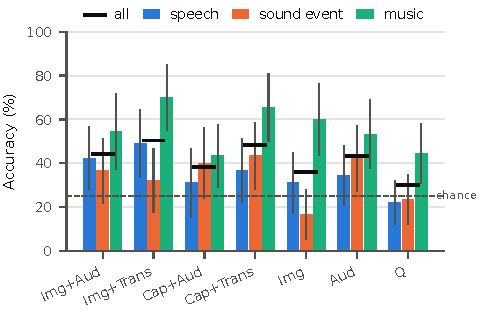
\includegraphics[width=\columnwidth]{figures/acc_by_config_audio.pdf}
\caption{Accuracy by input configuration and audio type (mean over three option orders), with 95\%
confidence intervals over items. Black ticks show the accuracy over all 90 items.}
\label{fig:app-acc-bars}
\end{figure}

\begin{table*}[t]
\caption{Full per-configuration results. Accuracy is shown both in the original option order and
averaged over three orders. Token counts and latency are means per item; \emph{Act.\ mem.} is the
activation memory (approximate on MPS); \emph{Max prob} is the mean probability of the predicted option.}
\label{tab:app-config}
\centering\small
\resizebox{\textwidth}{!}{%
\begin{tabular}{lccccccccc}
\toprule
Input & Acc.\ (orig.) & Acc.\ (avg.) & Image tok. & Audio tok. & Text tok. & Lat.\ mean (s) & Lat.\ p90 (s) & Act.\ mem.\ (MB) & Max prob \\
\midrule
Image+Audio        & 38.9 & 44.4 & 700 & 270 & 136 & 3.31 & 4.01 & 327 & .71 \\
Image+Transcript   & 47.8 & 50.4 & 700 &   0 & 161 & 2.66 & 3.00 & 255 & .76 \\
Caption+Audio      & 40.0 & 38.1 &   0 & 270 & 401 & 1.39 & 2.37 & 197 & .70 \\
Caption+Transcript & 46.7 & 48.5 &   0 &   0 & 427 & 0.77 & 0.95 & 126 & .72 \\
Image only         & 33.3 & 35.9 & 700 &   0 & 134 & 2.62 & 2.92 & 246 & .74 \\
Audio only         & 40.0 & 43.3 &   0 & 270 & 134 & 0.98 & 1.84 & 119 & .66 \\
Question only      & 30.0 & 30.0 &   0 &   0 & 132 & 0.31 & 0.39 &  39 & .52 \\
\bottomrule
\end{tabular}}
\end{table*}

\paragraph{Costs.} \Cref{tab:app-config} gives the full cost breakdown. Latency
and activation memory follow the token count closely, except that image tokens
are more expensive per token than text or audio tokens: image-only (834 tokens)
takes 2.6\,s, while caption+audio (671 tokens) takes 1.4\,s. This is because the
vision encoder runs on about four times as many patches before merging. A caption
costs 268 tokens on average but is much longer for music items, so on music the
cost advantage of caption+transcript shrinks.

\begin{table}[h]
\caption{Robustness to option order: accuracy in each order, the share of items answered correctly in
all three orders, and the share where the model gives the same answer in all three.}
\label{tab:app-perm}
\centering\small
\setlength{\tabcolsep}{3.5pt}
\begin{tabular}{lccccc}
\toprule
Input & Ord.\ 0 & Ord.\ 1 & Ord.\ 2 & All correct & Same answer \\
\midrule
Image+Audio        & 38.9 & 48.9 & 45.6 & 33.3 & 65.6 \\
Image+Transcript   & 47.8 & 54.4 & 48.9 & 40.0 & 71.1 \\
Caption+Audio      & 40.0 & 36.7 & 37.8 & 26.7 & 63.3 \\
Caption+Transcript & 46.7 & 48.9 & 50.0 & 35.6 & 62.2 \\
Image only         & 33.3 & 38.9 & 35.6 & 25.6 & 67.8 \\
Audio only         & 40.0 & 45.6 & 44.4 & 27.8 & 57.8 \\
Question only      & 30.0 & 33.3 & 26.7 & 11.1 & 33.3 \\
\bottomrule
\end{tabular}
\end{table}

\begin{table}[h]
\caption{Share of the model's predicted letters (\%, all orders) per configuration, vs.\ the share of
gold answers at each position in the original order.}
\label{tab:app-letters}
\centering\small
\begin{tabular}{lcccc}
\toprule
 & A & B & C & D \\
\midrule
Gold (original order, subset) & 8 & 27 & 22 & 43 \\
\midrule
Image+Audio        & 24 & 34 & 23 & 20 \\
Image+Transcript   & 27 & 32 & 21 & 20 \\
Caption+Audio      & 21 & 43 & 20 & 16 \\
Caption+Transcript & 21 & 44 & 17 & 19 \\
Image only         & 24 & 35 & 23 & 18 \\
Audio only         & 23 & 39 & 23 & 16 \\
Question only      & 23 & 49 & 19 &  9 \\
\bottomrule
\end{tabular}
\end{table}

\paragraph{Option-order effects.} \Cref{tab:app-perm} shows that accuracy can
move by up to 10 points between orders for the same configuration (Image+Audio:
38.9\% to 48.9\%), and that the model gives the same answer in all three orders
on only 58--71\% of items, or 33\% for question only, which is essentially guessing.
\Cref{tab:app-letters} shows the source: the model over-predicts ``B'' in every
configuration, most strongly when it has the least information (49\% for question
only), while the gold answers are concentrated at ``D''.

\begin{figure}[h]
\centering
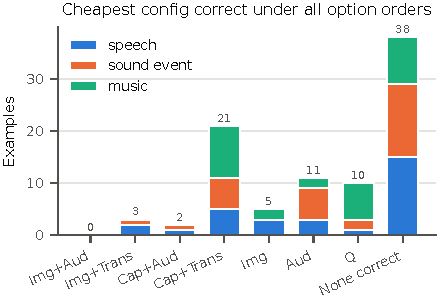
\includegraphics[width=\columnwidth]{figures/oracle_routing.pdf}
\caption{For each item, the cheapest configuration that is correct under all three option orders
(the permutation-robust oracle), stacked by audio type.}
\label{fig:app-oracle}
\end{figure}

\paragraph{Oracle routing.} \Cref{fig:app-oracle} shows which configuration the
permutation-robust oracle picks. Caption+transcript is the cheapest robust
solution for 21 items (10 of them music), audio only for 11 (6 sound events), and
question only for 10 (7 music). The full input is never the cheapest robust
solution, and 38 items (15 speech, 14 sound, 9 music) are not solved robustly by
any configuration. The oracle reaches 57.8\% accuracy at 25\% of the full-input
cost, whereas an oracle over the original order alone reports 68.9\% at 22\%,
inflated by lucky guesses.

\begin{figure}[h]
\centering
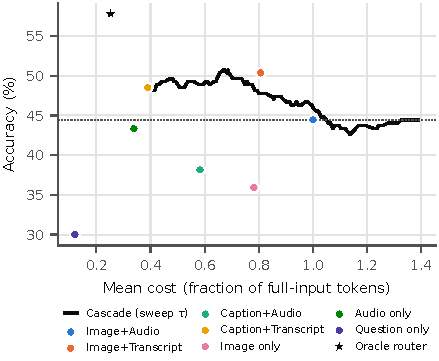
\includegraphics[width=\columnwidth]{figures/cascade.pdf}
\caption{Confidence cascade: answer from caption+transcript and escalate to the full input when the
maximum option probability is below $\tau$ (curve traced by sweeping $\tau$; accuracy averaged over
option orders). Points are the fixed configurations; the star is the permutation-robust oracle.}
\label{fig:app-cascade}
\end{figure}

\paragraph{Cascade.} \Cref{fig:app-cascade} traces the cascade as the threshold
$\tau$ varies. Escalating a few low-confidence items raises accuracy slightly
(peak 50.7\% at 67\% of the cost, $\tau{=}0.565$, escalating 28\% of items), but
escalating more lowers it toward the full-input level (44.4\%), because the full
input is not more accurate than caption+transcript. The cascade never reaches the
oracle; this gap is the headroom a learned router would need to close.

\begin{figure}[h]
\centering
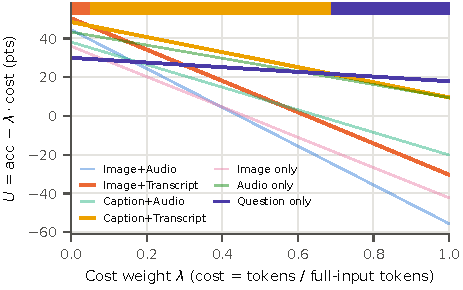
\includegraphics[width=\columnwidth]{figures/utility_sweep.pdf}
\caption{Utility $U{=}\text{acc}-\lambda\cdot\text{cost}$ per configuration as the cost weight $\lambda$
varies; the colored strip at the top marks the optimal configuration.}
\label{fig:app-utility}
\end{figure}

\paragraph{Utility sweep.} \Cref{fig:app-utility} shows which configuration is
optimal as cost is weighted more heavily. Image+transcript is optimal only when
cost barely matters ($\lambda\le0.04$), caption+transcript for
$0.05\le\lambda\le0.68$, and question only beyond that. A single fixed choice is
therefore near-optimal for most cost preferences, so a router's gains must come
from per-item decisions rather than from choosing a better global configuration.

% ---------------------------------------------------------------------
\subsection{Analysis 3: additional language results}
\label{app:a3}

\begin{figure*}[t]
\centering
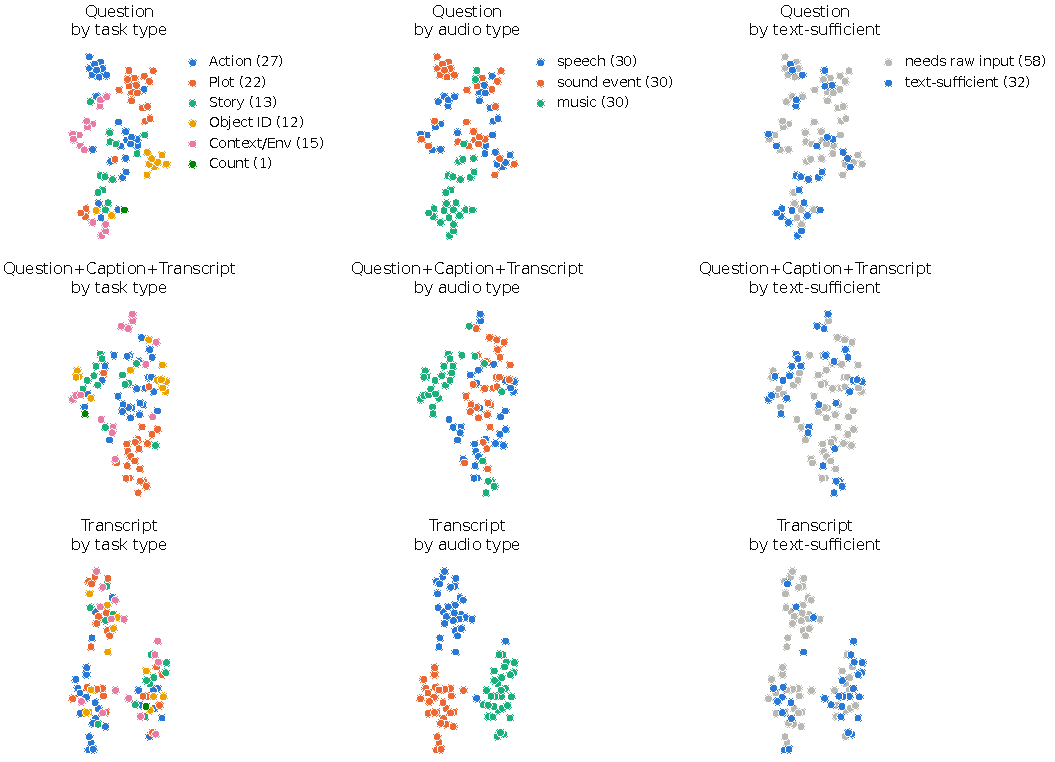
\includegraphics[width=\textwidth]{figures/tsne_grid.pdf}
\caption{t-SNE of SBERT embeddings for the three text views (rows), colored by task type, audio type,
and the model's text-sufficient label (columns). Counts are given in the legends.}
\label{fig:app-tsne-grid}
\end{figure*}

\begin{table}[h]
\caption{Cosine silhouette scores of each grouping in each embedding view (higher means the
grouping is more separated; about 0 means no separation).}
\label{tab:app-sil}
\centering\small
\setlength{\tabcolsep}{4pt}
\begin{tabular}{lcccc}
\toprule
View & Task & Audio & Text-suff.\ (model) & Text-suff.\ (human) \\
\midrule
Question                    & 0.12 & 0.06 & 0.01 & $-0.01$ \\
Question+Caption+Transcript & 0.04 & 0.07 & 0.01 & $-0.02$ \\
Transcript                  & $-0.09$ & 0.19 & 0.01 & $-0.01$ \\
\bottomrule
\end{tabular}
\end{table}

\paragraph{Embedding structure.} \Cref{fig:app-tsne-grid,tab:app-sil} extend
\cref{fig:tsne} to all three views. Question embeddings group mostly by task type
(e.g.\ ``what will happen next'' questions cluster together), transcript embeddings
by audio type, and the combined view shows weak structure for both. No view
separates text-sufficient items, under either model or human labels.

\begin{figure}[h]
\centering
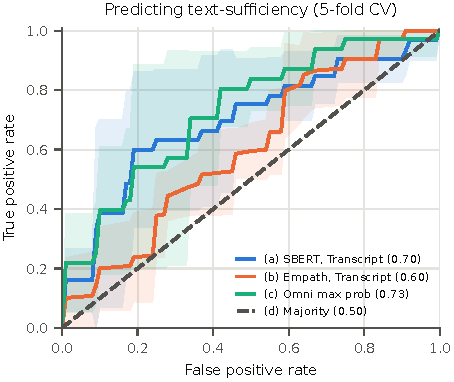
\includegraphics[width=\columnwidth]{figures/predict_roc.pdf}
\caption{Mean ROC curves over five folds (bands: $\pm$1 std) for the best view of each predictor
(model labels). AUROC in parentheses.}
\label{fig:app-roc}
\end{figure}

\begin{figure}[h]
\centering
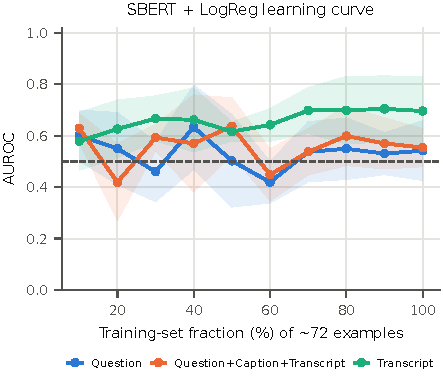
\includegraphics[width=\columnwidth]{figures/predict_learning_curve.pdf}
\caption{Learning curve of SBERT + logistic regression: AUROC on held-out folds when training on a
fraction of each training split (bands: $\pm$1 std over folds; model labels).}
\label{fig:app-lc}
\end{figure}

\paragraph{ROC and learning curves.} In \cref{fig:app-roc}, the model's
confidence and the transcript embeddings perform similarly at low false-positive
rates, and the confidence is better at moderate rates (0.35--0.7); Empath stays
close to chance below a false-positive rate of 0.25. Unlike the transcript
predictor, the confidence needs no training. In \cref{fig:app-lc}, only
the transcript view improves with more data (0.58 at 10\% to 0.70 at 100\%); the
question view stays near chance (0.60 to 0.54) and the combined view does not
improve (0.63 to 0.55). More data might help a transcript-based predictor
somewhat, but it would mostly learn the audio type.

\begin{figure}[h]
\centering
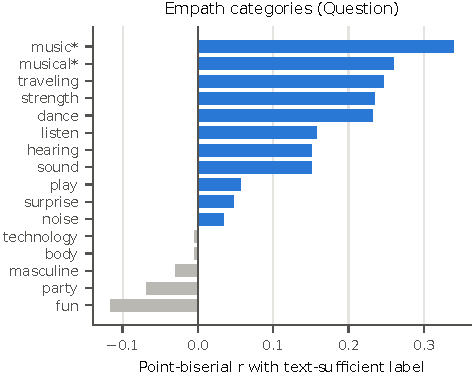
\includegraphics[width=\columnwidth]{figures/empath_top_question.pdf}
\caption{Empath categories in the question text most associated with the model's text-sufficient label
(point-biserial $r$). * marks Benjamini--Hochberg $q<0.05$ over 194 categories.}
\label{fig:app-empath}
\end{figure}

\paragraph{Empath.} \Cref{fig:app-empath} shows the strongest question-view
associations. Only \emph{music} and \emph{musical} survive correction, and the
next categories (\emph{dance}, \emph{listen}, \emph{hearing}, \emph{sound}) are also
audio-related. In the combined view the top categories (\emph{love}, \emph{fire},
\emph{beauty}; $r\approx0.27$--$0.30$) do not survive correction ($q\ge0.35$).
With human labels, nothing survives in any view (smallest $q{=}0.31$). The
interpretable features therefore recover the same signal as the embeddings,
namely the audio type, rather than identifying content that is answerable from
text.
).
% Needs: booktabs, multirow, graphicx (already loaded in main.tex).
% Figures: upload report/figures/*.pdf to the Overleaf "figures/" folder.
% Annotators are A1--A4, consistent with Table 1 in the main text.
% =====================================================================

\section{Supplementary Results}
\label{app:results}

This appendix reports results and implementation details that support the main
text but did not fit in the page limit. All numbers are regenerated by the
scripts in the repository (\texttt{src/analysis\_\{a,b,c\}/analyze.py},
\texttt{src/analysis\_c/predict.py}).

% ---------------------------------------------------------------------
\subsection{Implementation details}
\label{app:impl}

\paragraph{Subset.} 90 items sampled with seed 42, 30 per audio type. Item 1091
is excluded because two of its options are identical, which makes its correct
letter ambiguous. All three analyses use this subset; Analysis~1 uses 50 of the
90 items.

\paragraph{Model and prompt.} We use the text-output component (``thinker'') of
Qwen2.5-Omni-3B in bfloat16 with the default Qwen system prompt, on an Apple M2
Max (PyTorch 2.14.1 with the MPS backend, \texttt{transformers} 5.18.0). The user
turn contains the raw media (if any), then the surrogate lines
\texttt{Image description:~\ldots} and/or \texttt{Audio transcript/description:~\ldots}
(if any), then \texttt{Question:~\ldots}, the options \texttt{A.}--\texttt{D.}, and
the instruction \emph{``Answer with the option's letter from the given choices
directly.''} Images are resized with Qwen's own resizing to at most
$768\times28\times28$ pixels (at most 768 visual tokens; mean 700). Audio is
resampled to 16\,kHz mono and costs 25 tokens per second (mean 270 tokens).

\paragraph{Scoring.} One forward pass per input. We take the next-token logits
at the answer position, keep the four letter tokens (each A--D is a single
token), and apply a softmax. In a 55-pass check, the highest-scoring vocabulary
token was always one of the four letters, and greedy generation always began
with the argmax letter. For shuffled orders, probabilities are mapped back to the
original options before scoring correctness.

\paragraph{Option orders.} Order 0 is the original; orders 1 and 2 are random
permutations seeded by (seed, item, order) and redrawn until they differ from the
earlier orders. Every configuration is run under all three orders (1,890 forward
passes in total).

\paragraph{Cost measurements.} Input tokens are counted by modality directly
from the processed input ids; ``text'' tokens include the system prompt and chat
template (about 110 tokens per item). Latency covers the forward pass only, with
batch size 1, three warm-up passes, and device synchronization before and after.
PyTorch's MPS backend has no peak-memory counter, so a background thread samples
allocated memory every 2\,ms during each pass; we report the peak minus the
pre-pass baseline (activation memory), which is approximate. Model weights take
about 9.05\,GB.

% ---------------------------------------------------------------------
\subsection{Analysis 1: additional human results}
\label{app:a1}

\begin{table}[h]
\caption{Pairwise agreement on the 10 shared items (Cohen's $\kappa$).}
\label{tab:app-pairs}
\centering\small
\begin{tabular}{lcccc}
\toprule
 & \multicolumn{2}{c}{Final answer} & \multicolumn{2}{c}{``Text is enough''} \\
Pair & Agree & $\kappa$ & Agree & $\kappa$ \\
\midrule
A1--A2 & 40\% & 0.22 & 70\% & 0.44 \\
A1--A3 & 50\% & 0.35 & 60\% & 0.17 \\
A1--A4 & 40\% & 0.20 & 80\% & 0.55 \\
A2--A3 & 50\% & 0.32 & 30\% & $-0.30$ \\
A2--A4 & 40\% & 0.24 & 50\% & 0.19 \\
A3--A4 & 30\% & 0.05 & 40\% & $-0.36$ \\
\midrule
All four (Fleiss) & -- & 0.22 & -- & 0.08 \\
\bottomrule
\end{tabular}
\end{table}

\begin{table}[h]
\caption{The 10 shared items: how many of the four annotators answered correctly, how many distinct
final answers they gave, and how many judged the text sufficient.}
\label{tab:app-shared}
\centering\small
\setlength{\tabcolsep}{4pt}
\begin{tabular}{rllcccc}
\toprule
Item & Audio & Task & Gold & Correct & Distinct & Text enough \\
\midrule
66   & speech & Action      & D & 0/4 & 3 & 3/4 \\
323  & speech & Plot        & D & 1/4 & 3 & 3/4 \\
389  & speech & Plot        & A & 0/4 & 2 & 1/4 \\
641  & speech & Context     & C & 3/4 & 2 & 1/4 \\
745  & sound  & Action      & C & 1/4 & 2 & 3/4 \\
847  & sound  & Story       & D & 3/4 & 2 & 1/4 \\
1019 & sound  & Action      & C & 2/4 & 3 & 1/4 \\
1057 & music  & Object ID   & C & 1/4 & 3 & 3/4 \\
1070 & music  & Story       & B & 4/4 & 1 & 4/4 \\
1086 & music  & Action      & B & 0/4 & 2 & 3/4 \\
\bottomrule
\end{tabular}
\end{table}

\paragraph{Agreement.} \Cref{tab:app-pairs,tab:app-shared} break down the low
agreement reported in \cref{sec:a1}. Agreement on the final answer is uniformly
low (30--50\% per pair), and agreement on ``text is enough'' is inconsistent:
some pairs agree reasonably (A1--A4, $\kappa{=}0.55$) while others disagree more
than chance would predict (A3--A4, $\kappa{=}-0.36$). Three shared items were
answered correctly by nobody, and on two of them most annotators had judged the
text sufficient, which illustrates the overconfidence in \cref{tab:annotators}.
Only item 1070 was answered correctly and unanimously.

\begin{table}[h]
\caption{Human results by audio type and task type (80 annotations). \emph{Text}: accuracy of stage-0
text-only answers; \emph{Final}: after revealing.}
\label{tab:app-human-breakdown}
\centering\small
\setlength{\tabcolsep}{4pt}
\begin{tabular}{lcccc}
\toprule
 & $n$ & Said enough & Text & Final \\
\midrule
Speech      & 29 & 62\% & 38\% & 41\% \\
Sound event & 26 & 62\% & 32\% & 54\% \\
Music       & 25 & 64\% & 45\% & 40\% \\
\midrule
Action and Activity          & 30 & 60\% & 19\% & 40\% \\
Plot Inference               & 18 & 61\% & 50\% & 44\% \\
Story Description            & 14 & 57\% & 50\% & 57\% \\
Contextual / Environmental   &  9 & 56\% & 44\% & 56\% \\
Object Identification        &  9 & 89\% & 44\% & 33\% \\
\bottomrule
\end{tabular}
\end{table}

\paragraph{By audio and task type.} \Cref{tab:app-human-breakdown} is in line
with H1.2: revealing the raw inputs helped most for sound events (32\% $\to$
54\%), whose transcripts are short descriptions, and for action questions
(19\% $\to$ 40\%). It did not help for music (45\% $\to$ 40\%). Annotators judged
text sufficient at similar rates for every audio type (62--64\%), even though
text-only accuracy differed. With 9--30 annotations per row, these breakdowns are
descriptive only.

\paragraph{Reveal behavior and cost.} Annotators revealed both modalities in 79
of 80 items and revealed the image first in 78. As a result, the token cost of
their information use (computed from each item's per-modality token counts in
Analysis~2) was uninformative: the mean was 1.26$\times$ the full-input cost,
since they read the caption and transcript as well as viewing both raw inputs.
Free-text notes named the audio as decisive in 33 annotations, the image in 31,
and the text in 26 (multiple labels allowed).

% ---------------------------------------------------------------------
\subsection{Analysis 2: additional model results}
\label{app:a2}

\begin{figure}[h]
\centering
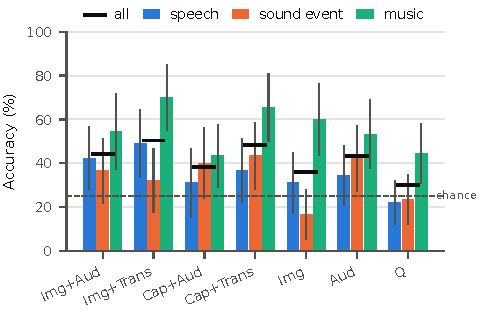
\includegraphics[width=\columnwidth]{figures/acc_by_config_audio.pdf}
\caption{Accuracy by input configuration and audio type (mean over three option orders), with 95\%
confidence intervals over items. Black ticks show the accuracy over all 90 items.}
\label{fig:app-acc-bars}
\end{figure}

\begin{table*}[t]
\caption{Full per-configuration results. Accuracy is shown both in the original option order and
averaged over three orders. Token counts and latency are means per item; \emph{Act.\ mem.} is the
activation memory (approximate on MPS); \emph{Max prob} is the mean probability of the predicted option.}
\label{tab:app-config}
\centering\small
\resizebox{\textwidth}{!}{%
\begin{tabular}{lccccccccc}
\toprule
Input & Acc.\ (orig.) & Acc.\ (avg.) & Image tok. & Audio tok. & Text tok. & Lat.\ mean (s) & Lat.\ p90 (s) & Act.\ mem.\ (MB) & Max prob \\
\midrule
Image+Audio        & 38.9 & 44.4 & 700 & 270 & 136 & 3.31 & 4.01 & 327 & .71 \\
Image+Transcript   & 47.8 & 50.4 & 700 &   0 & 161 & 2.66 & 3.00 & 255 & .76 \\
Caption+Audio      & 40.0 & 38.1 &   0 & 270 & 401 & 1.39 & 2.37 & 197 & .70 \\
Caption+Transcript & 46.7 & 48.5 &   0 &   0 & 427 & 0.77 & 0.95 & 126 & .72 \\
Image only         & 33.3 & 35.9 & 700 &   0 & 134 & 2.62 & 2.92 & 246 & .74 \\
Audio only         & 40.0 & 43.3 &   0 & 270 & 134 & 0.98 & 1.84 & 119 & .66 \\
Question only      & 30.0 & 30.0 &   0 &   0 & 132 & 0.31 & 0.39 &  39 & .52 \\
\bottomrule
\end{tabular}}
\end{table*}

\paragraph{Costs.} \Cref{tab:app-config} gives the full cost breakdown. Latency
and activation memory follow the token count closely, except that image tokens
are more expensive per token than text or audio tokens: image-only (834 tokens)
takes 2.6\,s, while caption+audio (671 tokens) takes 1.4\,s. This is because the
vision encoder runs on about four times as many patches before merging. A caption
costs 268 tokens on average but is much longer for music items, so on music the
cost advantage of caption+transcript shrinks.

\begin{table}[h]
\caption{Robustness to option order: accuracy in each order, the share of items answered correctly in
all three orders, and the share where the model gives the same answer in all three.}
\label{tab:app-perm}
\centering\small
\setlength{\tabcolsep}{3.5pt}
\begin{tabular}{lccccc}
\toprule
Input & Ord.\ 0 & Ord.\ 1 & Ord.\ 2 & All correct & Same answer \\
\midrule
Image+Audio        & 38.9 & 48.9 & 45.6 & 33.3 & 65.6 \\
Image+Transcript   & 47.8 & 54.4 & 48.9 & 40.0 & 71.1 \\
Caption+Audio      & 40.0 & 36.7 & 37.8 & 26.7 & 63.3 \\
Caption+Transcript & 46.7 & 48.9 & 50.0 & 35.6 & 62.2 \\
Image only         & 33.3 & 38.9 & 35.6 & 25.6 & 67.8 \\
Audio only         & 40.0 & 45.6 & 44.4 & 27.8 & 57.8 \\
Question only      & 30.0 & 33.3 & 26.7 & 11.1 & 33.3 \\
\bottomrule
\end{tabular}
\end{table}

\begin{table}[h]
\caption{Share of the model's predicted letters (\%, all orders) per configuration, vs.\ the share of
gold answers at each position in the original order.}
\label{tab:app-letters}
\centering\small
\begin{tabular}{lcccc}
\toprule
 & A & B & C & D \\
\midrule
Gold (original order, subset) & 8 & 27 & 22 & 43 \\
\midrule
Image+Audio        & 24 & 34 & 23 & 20 \\
Image+Transcript   & 27 & 32 & 21 & 20 \\
Caption+Audio      & 21 & 43 & 20 & 16 \\
Caption+Transcript & 21 & 44 & 17 & 19 \\
Image only         & 24 & 35 & 23 & 18 \\
Audio only         & 23 & 39 & 23 & 16 \\
Question only      & 23 & 49 & 19 &  9 \\
\bottomrule
\end{tabular}
\end{table}

\paragraph{Option-order effects.} \Cref{tab:app-perm} shows that accuracy can
move by up to 10 points between orders for the same configuration (Image+Audio:
38.9\% to 48.9\%), and that the model gives the same answer in all three orders
on only 58--71\% of items, or 33\% for question only, which is essentially guessing.
\Cref{tab:app-letters} shows the source: the model over-predicts ``B'' in every
configuration, most strongly when it has the least information (49\% for question
only), while the gold answers are concentrated at ``D''.

\begin{figure}[h]
\centering
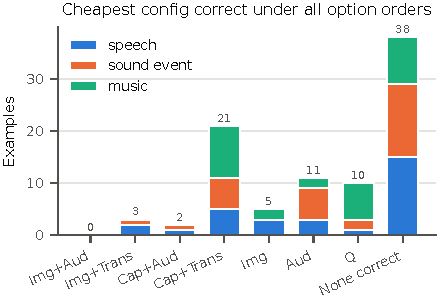
\includegraphics[width=\columnwidth]{figures/oracle_routing.pdf}
\caption{For each item, the cheapest configuration that is correct under all three option orders
(the permutation-robust oracle), stacked by audio type.}
\label{fig:app-oracle}
\end{figure}

\paragraph{Oracle routing.} \Cref{fig:app-oracle} shows which configuration the
permutation-robust oracle picks. Caption+transcript is the cheapest robust
solution for 21 items (10 of them music), audio only for 11 (6 sound events), and
question only for 10 (7 music). The full input is never the cheapest robust
solution, and 38 items (15 speech, 14 sound, 9 music) are not solved robustly by
any configuration. The oracle reaches 57.8\% accuracy at 25\% of the full-input
cost, whereas an oracle over the original order alone reports 68.9\% at 22\%,
inflated by lucky guesses.

\begin{figure}[h]
\centering
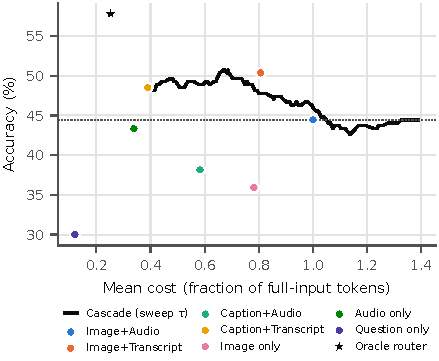
\includegraphics[width=\columnwidth]{figures/cascade.pdf}
\caption{Confidence cascade: answer from caption+transcript and escalate to the full input when the
maximum option probability is below $\tau$ (curve traced by sweeping $\tau$; accuracy averaged over
option orders). Points are the fixed configurations; the star is the permutation-robust oracle.}
\label{fig:app-cascade}
\end{figure}

\paragraph{Cascade.} \Cref{fig:app-cascade} traces the cascade as the threshold
$\tau$ varies. Escalating a few low-confidence items raises accuracy slightly
(peak 50.7\% at 67\% of the cost, $\tau{=}0.565$, escalating 28\% of items), but
escalating more lowers it toward the full-input level (44.4\%), because the full
input is not more accurate than caption+transcript. The cascade never reaches the
oracle; this gap is the headroom a learned router would need to close.

\begin{figure}[h]
\centering
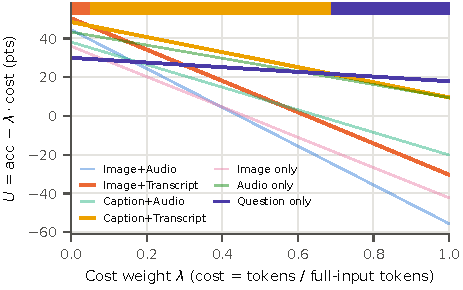
\includegraphics[width=\columnwidth]{figures/utility_sweep.pdf}
\caption{Utility $U{=}\text{acc}-\lambda\cdot\text{cost}$ per configuration as the cost weight $\lambda$
varies; the colored strip at the top marks the optimal configuration.}
\label{fig:app-utility}
\end{figure}

\paragraph{Utility sweep.} \Cref{fig:app-utility} shows which configuration is
optimal as cost is weighted more heavily. Image+transcript is optimal only when
cost barely matters ($\lambda\le0.04$), caption+transcript for
$0.05\le\lambda\le0.68$, and question only beyond that. A single fixed choice is
therefore near-optimal for most cost preferences, so a router's gains must come
from per-item decisions rather than from choosing a better global configuration.

% ---------------------------------------------------------------------
\subsection{Analysis 3: additional language results}
\label{app:a3}

\begin{figure*}[t]
\centering
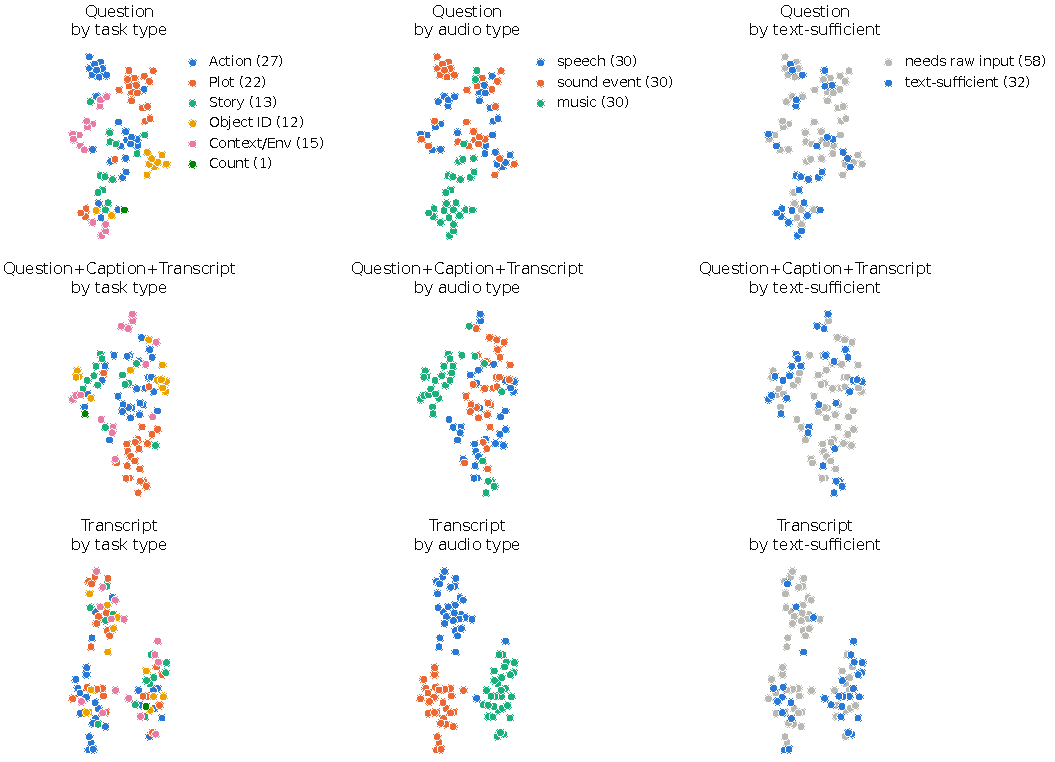
\includegraphics[width=\textwidth]{figures/tsne_grid.pdf}
\caption{t-SNE of SBERT embeddings for the three text views (rows), colored by task type, audio type,
and the model's text-sufficient label (columns). Counts are given in the legends.}
\label{fig:app-tsne-grid}
\end{figure*}

\begin{table}[h]
\caption{Cosine silhouette scores of each grouping in each embedding view (higher means the
grouping is more separated; about 0 means no separation).}
\label{tab:app-sil}
\centering\small
\setlength{\tabcolsep}{4pt}
\begin{tabular}{lcccc}
\toprule
View & Task & Audio & Text-suff.\ (model) & Text-suff.\ (human) \\
\midrule
Question                    & 0.12 & 0.06 & 0.01 & $-0.01$ \\
Question+Caption+Transcript & 0.04 & 0.07 & 0.01 & $-0.02$ \\
Transcript                  & $-0.09$ & 0.19 & 0.01 & $-0.01$ \\
\bottomrule
\end{tabular}
\end{table}

\paragraph{Embedding structure.} \Cref{fig:app-tsne-grid,tab:app-sil} extend
\cref{fig:tsne} to all three views. Question embeddings group mostly by task type
(e.g.\ ``what will happen next'' questions cluster together), transcript embeddings
by audio type, and the combined view shows weak structure for both. No view
separates text-sufficient items, under either model or human labels.

\begin{figure}[h]
\centering
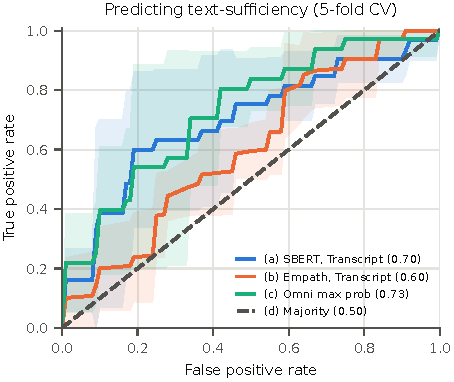
\includegraphics[width=\columnwidth]{figures/predict_roc.pdf}
\caption{Mean ROC curves over five folds (bands: $\pm$1 std) for the best view of each predictor
(model labels). AUROC in parentheses.}
\label{fig:app-roc}
\end{figure}

\begin{figure}[h]
\centering
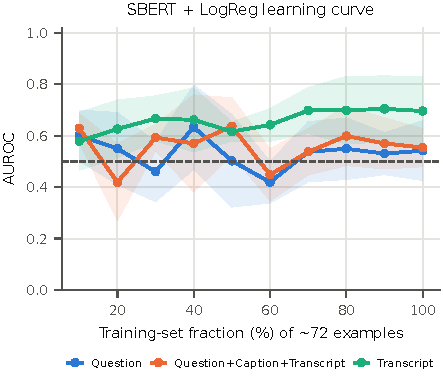
\includegraphics[width=\columnwidth]{figures/predict_learning_curve.pdf}
\caption{Learning curve of SBERT + logistic regression: AUROC on held-out folds when training on a
fraction of each training split (bands: $\pm$1 std over folds; model labels).}
\label{fig:app-lc}
\end{figure}

\paragraph{ROC and learning curves.} In \cref{fig:app-roc}, the model's
confidence and the transcript embeddings perform similarly at low false-positive
rates, and the confidence is better at moderate rates (0.35--0.7); Empath stays
close to chance below a false-positive rate of 0.25. Unlike the transcript
predictor, the confidence needs no training. In \cref{fig:app-lc}, only
the transcript view improves with more data (0.58 at 10\% to 0.70 at 100\%); the
question view stays near chance (0.60 to 0.54) and the combined view does not
improve (0.63 to 0.55). More data might help a transcript-based predictor
somewhat, but it would mostly learn the audio type.

\begin{figure}[h]
\centering
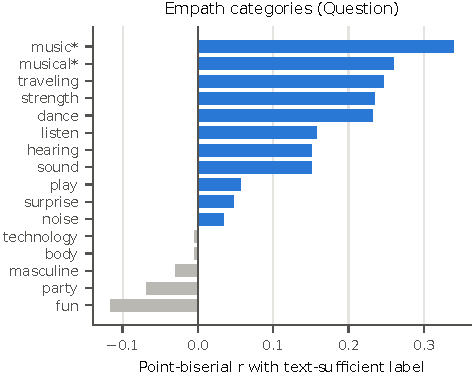
\includegraphics[width=\columnwidth]{figures/empath_top_question.pdf}
\caption{Empath categories in the question text most associated with the model's text-sufficient label
(point-biserial $r$). * marks Benjamini--Hochberg $q<0.05$ over 194 categories.}
\label{fig:app-empath}
\end{figure}

\paragraph{Empath.} \Cref{fig:app-empath} shows the strongest question-view
associations. Only \emph{music} and \emph{musical} survive correction, and the
next categories (\emph{dance}, \emph{listen}, \emph{hearing}, \emph{sound}) are also
audio-related. In the combined view the top categories (\emph{love}, \emph{fire},
\emph{beauty}; $r\approx0.27$--$0.30$) do not survive correction ($q\ge0.35$).
With human labels, nothing survives in any view (smallest $q{=}0.31$). The
interpretable features therefore recover the same signal as the embeddings,
namely the audio type, rather than identifying content that is answerable from
text.
).
% Needs: booktabs, multirow, graphicx (already loaded in main.tex).
% Figures: upload report/figures/*.pdf to the Overleaf "figures/" folder.
% Annotators are A1--A4, consistent with Table 1 in the main text.
% =====================================================================

\section{Supplementary Results}
\label{app:results}

This appendix reports results and implementation details that support the main
text but did not fit in the page limit. All numbers are regenerated by the
scripts in the repository (\texttt{src/analysis\_\{a,b,c\}/analyze.py},
\texttt{src/analysis\_c/predict.py}).

% ---------------------------------------------------------------------
\subsection{Implementation details}
\label{app:impl}

\paragraph{Subset.} 90 items sampled with seed 42, 30 per audio type. Item 1091
is excluded because two of its options are identical, which makes its correct
letter ambiguous. All three analyses use this subset; Analysis~1 uses 50 of the
90 items.

\paragraph{Model and prompt.} We use the text-output component (``thinker'') of
Qwen2.5-Omni-3B in bfloat16 with the default Qwen system prompt, on an Apple M2
Max (PyTorch 2.14.1 with the MPS backend, \texttt{transformers} 5.18.0). The user
turn contains the raw media (if any), then the surrogate lines
\texttt{Image description:~\ldots} and/or \texttt{Audio transcript/description:~\ldots}
(if any), then \texttt{Question:~\ldots}, the options \texttt{A.}--\texttt{D.}, and
the instruction \emph{``Answer with the option's letter from the given choices
directly.''} Images are resized with Qwen's own resizing to at most
$768\times28\times28$ pixels (at most 768 visual tokens; mean 700). Audio is
resampled to 16\,kHz mono and costs 25 tokens per second (mean 270 tokens).

\paragraph{Scoring.} One forward pass per input. We take the next-token logits
at the answer position, keep the four letter tokens (each A--D is a single
token), and apply a softmax. In a 55-pass check, the highest-scoring vocabulary
token was always one of the four letters, and greedy generation always began
with the argmax letter. For shuffled orders, probabilities are mapped back to the
original options before scoring correctness.

\paragraph{Option orders.} Order 0 is the original; orders 1 and 2 are random
permutations seeded by (seed, item, order) and redrawn until they differ from the
earlier orders. Every configuration is run under all three orders (1,890 forward
passes in total).

\paragraph{Cost measurements.} Input tokens are counted by modality directly
from the processed input ids; ``text'' tokens include the system prompt and chat
template (about 110 tokens per item). Latency covers the forward pass only, with
batch size 1, three warm-up passes, and device synchronization before and after.
PyTorch's MPS backend has no peak-memory counter, so a background thread samples
allocated memory every 2\,ms during each pass; we report the peak minus the
pre-pass baseline (activation memory), which is approximate. Model weights take
about 9.05\,GB.

% ---------------------------------------------------------------------
\subsection{Analysis 1: additional human results}
\label{app:a1}

\begin{table}[h]
\caption{Pairwise agreement on the 10 shared items (Cohen's $\kappa$).}
\label{tab:app-pairs}
\centering\small
\begin{tabular}{lcccc}
\toprule
 & \multicolumn{2}{c}{Final answer} & \multicolumn{2}{c}{``Text is enough''} \\
Pair & Agree & $\kappa$ & Agree & $\kappa$ \\
\midrule
A1--A2 & 40\% & 0.22 & 70\% & 0.44 \\
A1--A3 & 50\% & 0.35 & 60\% & 0.17 \\
A1--A4 & 40\% & 0.20 & 80\% & 0.55 \\
A2--A3 & 50\% & 0.32 & 30\% & $-0.30$ \\
A2--A4 & 40\% & 0.24 & 50\% & 0.19 \\
A3--A4 & 30\% & 0.05 & 40\% & $-0.36$ \\
\midrule
All four (Fleiss) & -- & 0.22 & -- & 0.08 \\
\bottomrule
\end{tabular}
\end{table}

\begin{table}[h]
\caption{The 10 shared items: how many of the four annotators answered correctly, how many distinct
final answers they gave, and how many judged the text sufficient.}
\label{tab:app-shared}
\centering\small
\setlength{\tabcolsep}{4pt}
\begin{tabular}{rllcccc}
\toprule
Item & Audio & Task & Gold & Correct & Distinct & Text enough \\
\midrule
66   & speech & Action      & D & 0/4 & 3 & 3/4 \\
323  & speech & Plot        & D & 1/4 & 3 & 3/4 \\
389  & speech & Plot        & A & 0/4 & 2 & 1/4 \\
641  & speech & Context     & C & 3/4 & 2 & 1/4 \\
745  & sound  & Action      & C & 1/4 & 2 & 3/4 \\
847  & sound  & Story       & D & 3/4 & 2 & 1/4 \\
1019 & sound  & Action      & C & 2/4 & 3 & 1/4 \\
1057 & music  & Object ID   & C & 1/4 & 3 & 3/4 \\
1070 & music  & Story       & B & 4/4 & 1 & 4/4 \\
1086 & music  & Action      & B & 0/4 & 2 & 3/4 \\
\bottomrule
\end{tabular}
\end{table}

\paragraph{Agreement.} \Cref{tab:app-pairs,tab:app-shared} break down the low
agreement reported in \cref{sec:a1}. Agreement on the final answer is uniformly
low (30--50\% per pair), and agreement on ``text is enough'' is inconsistent:
some pairs agree reasonably (A1--A4, $\kappa{=}0.55$) while others disagree more
than chance would predict (A3--A4, $\kappa{=}-0.36$). Three shared items were
answered correctly by nobody, and on two of them most annotators had judged the
text sufficient, which illustrates the overconfidence in \cref{tab:annotators}.
Only item 1070 was answered correctly and unanimously.

\begin{table}[h]
\caption{Human results by audio type and task type (80 annotations). \emph{Text}: accuracy of stage-0
text-only answers; \emph{Final}: after revealing.}
\label{tab:app-human-breakdown}
\centering\small
\setlength{\tabcolsep}{4pt}
\begin{tabular}{lcccc}
\toprule
 & $n$ & Said enough & Text & Final \\
\midrule
Speech      & 29 & 62\% & 38\% & 41\% \\
Sound event & 26 & 62\% & 32\% & 54\% \\
Music       & 25 & 64\% & 45\% & 40\% \\
\midrule
Action and Activity          & 30 & 60\% & 19\% & 40\% \\
Plot Inference               & 18 & 61\% & 50\% & 44\% \\
Story Description            & 14 & 57\% & 50\% & 57\% \\
Contextual / Environmental   &  9 & 56\% & 44\% & 56\% \\
Object Identification        &  9 & 89\% & 44\% & 33\% \\
\bottomrule
\end{tabular}
\end{table}

\paragraph{By audio and task type.} \Cref{tab:app-human-breakdown} is in line
with H1.2: revealing the raw inputs helped most for sound events (32\% $\to$
54\%), whose transcripts are short descriptions, and for action questions
(19\% $\to$ 40\%). It did not help for music (45\% $\to$ 40\%). Annotators judged
text sufficient at similar rates for every audio type (62--64\%), even though
text-only accuracy differed. With 9--30 annotations per row, these breakdowns are
descriptive only.

\paragraph{Reveal behavior and cost.} Annotators revealed both modalities in 79
of 80 items and revealed the image first in 78. As a result, the token cost of
their information use (computed from each item's per-modality token counts in
Analysis~2) was uninformative: the mean was 1.26$\times$ the full-input cost,
since they read the caption and transcript as well as viewing both raw inputs.
Free-text notes named the audio as decisive in 33 annotations, the image in 31,
and the text in 26 (multiple labels allowed).

% ---------------------------------------------------------------------
\subsection{Analysis 2: additional model results}
\label{app:a2}

\begin{figure}[h]
\centering
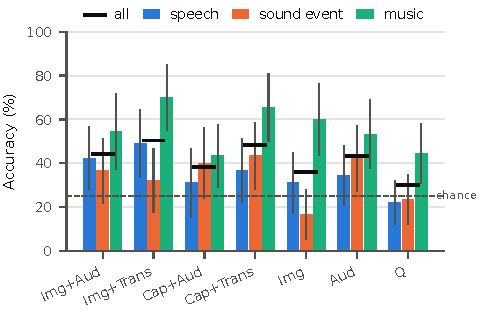
\includegraphics[width=\columnwidth]{figures/acc_by_config_audio.pdf}
\caption{Accuracy by input configuration and audio type (mean over three option orders), with 95\%
confidence intervals over items. Black ticks show the accuracy over all 90 items.}
\label{fig:app-acc-bars}
\end{figure}

\begin{table*}[t]
\caption{Full per-configuration results. Accuracy is shown both in the original option order and
averaged over three orders. Token counts and latency are means per item; \emph{Act.\ mem.} is the
activation memory (approximate on MPS); \emph{Max prob} is the mean probability of the predicted option.}
\label{tab:app-config}
\centering\small
\resizebox{\textwidth}{!}{%
\begin{tabular}{lccccccccc}
\toprule
Input & Acc.\ (orig.) & Acc.\ (avg.) & Image tok. & Audio tok. & Text tok. & Lat.\ mean (s) & Lat.\ p90 (s) & Act.\ mem.\ (MB) & Max prob \\
\midrule
Image+Audio        & 38.9 & 44.4 & 700 & 270 & 136 & 3.31 & 4.01 & 327 & .71 \\
Image+Transcript   & 47.8 & 50.4 & 700 &   0 & 161 & 2.66 & 3.00 & 255 & .76 \\
Caption+Audio      & 40.0 & 38.1 &   0 & 270 & 401 & 1.39 & 2.37 & 197 & .70 \\
Caption+Transcript & 46.7 & 48.5 &   0 &   0 & 427 & 0.77 & 0.95 & 126 & .72 \\
Image only         & 33.3 & 35.9 & 700 &   0 & 134 & 2.62 & 2.92 & 246 & .74 \\
Audio only         & 40.0 & 43.3 &   0 & 270 & 134 & 0.98 & 1.84 & 119 & .66 \\
Question only      & 30.0 & 30.0 &   0 &   0 & 132 & 0.31 & 0.39 &  39 & .52 \\
\bottomrule
\end{tabular}}
\end{table*}

\paragraph{Costs.} \Cref{tab:app-config} gives the full cost breakdown. Latency
and activation memory follow the token count closely, except that image tokens
are more expensive per token than text or audio tokens: image-only (834 tokens)
takes 2.6\,s, while caption+audio (671 tokens) takes 1.4\,s. This is because the
vision encoder runs on about four times as many patches before merging. A caption
costs 268 tokens on average but is much longer for music items, so on music the
cost advantage of caption+transcript shrinks.

\begin{table}[h]
\caption{Robustness to option order: accuracy in each order, the share of items answered correctly in
all three orders, and the share where the model gives the same answer in all three.}
\label{tab:app-perm}
\centering\small
\setlength{\tabcolsep}{3.5pt}
\begin{tabular}{lccccc}
\toprule
Input & Ord.\ 0 & Ord.\ 1 & Ord.\ 2 & All correct & Same answer \\
\midrule
Image+Audio        & 38.9 & 48.9 & 45.6 & 33.3 & 65.6 \\
Image+Transcript   & 47.8 & 54.4 & 48.9 & 40.0 & 71.1 \\
Caption+Audio      & 40.0 & 36.7 & 37.8 & 26.7 & 63.3 \\
Caption+Transcript & 46.7 & 48.9 & 50.0 & 35.6 & 62.2 \\
Image only         & 33.3 & 38.9 & 35.6 & 25.6 & 67.8 \\
Audio only         & 40.0 & 45.6 & 44.4 & 27.8 & 57.8 \\
Question only      & 30.0 & 33.3 & 26.7 & 11.1 & 33.3 \\
\bottomrule
\end{tabular}
\end{table}

\begin{table}[h]
\caption{Share of the model's predicted letters (\%, all orders) per configuration, vs.\ the share of
gold answers at each position in the original order.}
\label{tab:app-letters}
\centering\small
\begin{tabular}{lcccc}
\toprule
 & A & B & C & D \\
\midrule
Gold (original order, subset) & 8 & 27 & 22 & 43 \\
\midrule
Image+Audio        & 24 & 34 & 23 & 20 \\
Image+Transcript   & 27 & 32 & 21 & 20 \\
Caption+Audio      & 21 & 43 & 20 & 16 \\
Caption+Transcript & 21 & 44 & 17 & 19 \\
Image only         & 24 & 35 & 23 & 18 \\
Audio only         & 23 & 39 & 23 & 16 \\
Question only      & 23 & 49 & 19 &  9 \\
\bottomrule
\end{tabular}
\end{table}

\paragraph{Option-order effects.} \Cref{tab:app-perm} shows that accuracy can
move by up to 10 points between orders for the same configuration (Image+Audio:
38.9\% to 48.9\%), and that the model gives the same answer in all three orders
on only 58--71\% of items, or 33\% for question only, which is essentially guessing.
\Cref{tab:app-letters} shows the source: the model over-predicts ``B'' in every
configuration, most strongly when it has the least information (49\% for question
only), while the gold answers are concentrated at ``D''.

\begin{figure}[h]
\centering
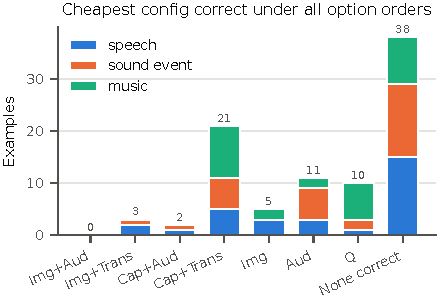
\includegraphics[width=\columnwidth]{figures/oracle_routing.pdf}
\caption{For each item, the cheapest configuration that is correct under all three option orders
(the permutation-robust oracle), stacked by audio type.}
\label{fig:app-oracle}
\end{figure}

\paragraph{Oracle routing.} \Cref{fig:app-oracle} shows which configuration the
permutation-robust oracle picks. Caption+transcript is the cheapest robust
solution for 21 items (10 of them music), audio only for 11 (6 sound events), and
question only for 10 (7 music). The full input is never the cheapest robust
solution, and 38 items (15 speech, 14 sound, 9 music) are not solved robustly by
any configuration. The oracle reaches 57.8\% accuracy at 25\% of the full-input
cost, whereas an oracle over the original order alone reports 68.9\% at 22\%,
inflated by lucky guesses.

\begin{figure}[h]
\centering
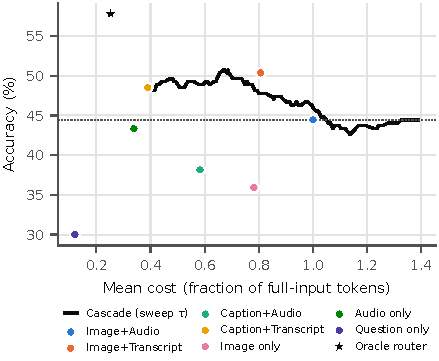
\includegraphics[width=\columnwidth]{figures/cascade.pdf}
\caption{Confidence cascade: answer from caption+transcript and escalate to the full input when the
maximum option probability is below $\tau$ (curve traced by sweeping $\tau$; accuracy averaged over
option orders). Points are the fixed configurations; the star is the permutation-robust oracle.}
\label{fig:app-cascade}
\end{figure}

\paragraph{Cascade.} \Cref{fig:app-cascade} traces the cascade as the threshold
$\tau$ varies. Escalating a few low-confidence items raises accuracy slightly
(peak 50.7\% at 67\% of the cost, $\tau{=}0.565$, escalating 28\% of items), but
escalating more lowers it toward the full-input level (44.4\%), because the full
input is not more accurate than caption+transcript. The cascade never reaches the
oracle; this gap is the headroom a learned router would need to close.

\begin{figure}[h]
\centering
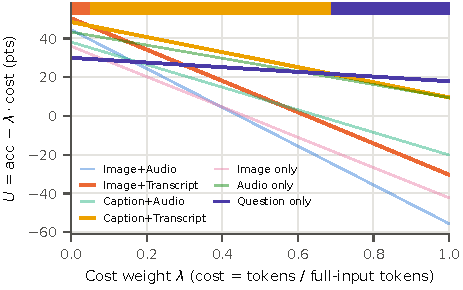
\includegraphics[width=\columnwidth]{figures/utility_sweep.pdf}
\caption{Utility $U{=}\text{acc}-\lambda\cdot\text{cost}$ per configuration as the cost weight $\lambda$
varies; the colored strip at the top marks the optimal configuration.}
\label{fig:app-utility}
\end{figure}

\paragraph{Utility sweep.} \Cref{fig:app-utility} shows which configuration is
optimal as cost is weighted more heavily. Image+transcript is optimal only when
cost barely matters ($\lambda\le0.04$), caption+transcript for
$0.05\le\lambda\le0.68$, and question only beyond that. A single fixed choice is
therefore near-optimal for most cost preferences, so a router's gains must come
from per-item decisions rather than from choosing a better global configuration.

% ---------------------------------------------------------------------
\subsection{Analysis 3: additional language results}
\label{app:a3}

\begin{figure*}[t]
\centering
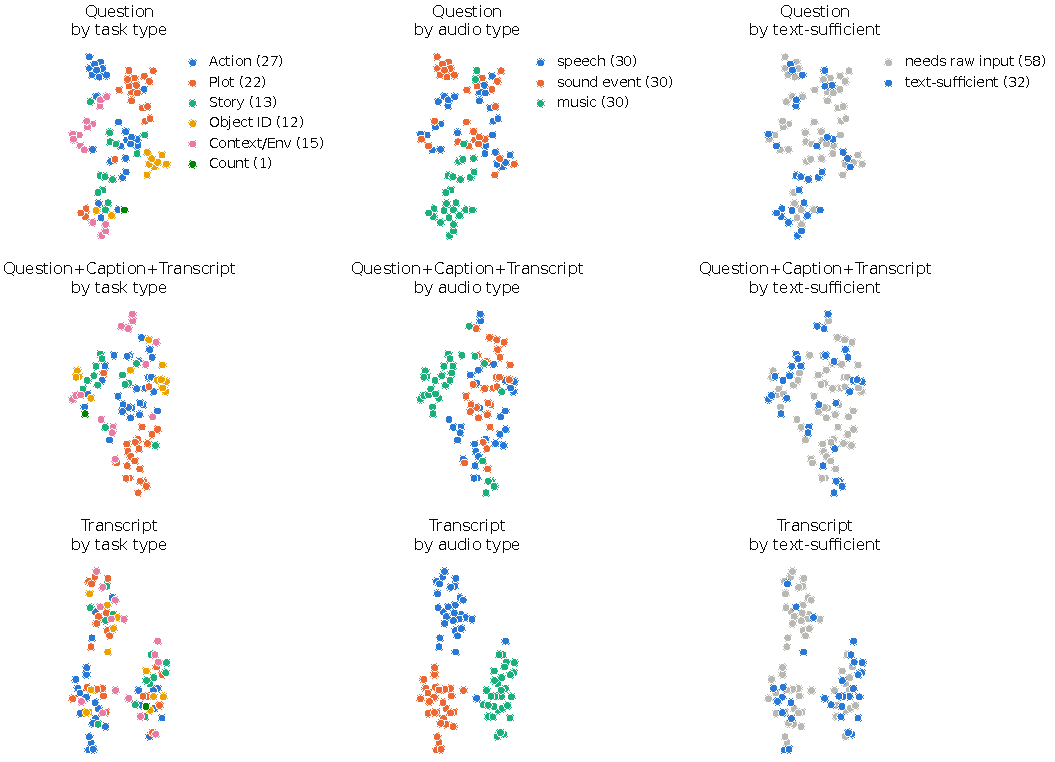
\includegraphics[width=\textwidth]{figures/tsne_grid.pdf}
\caption{t-SNE of SBERT embeddings for the three text views (rows), colored by task type, audio type,
and the model's text-sufficient label (columns). Counts are given in the legends.}
\label{fig:app-tsne-grid}
\end{figure*}

\begin{table}[h]
\caption{Cosine silhouette scores of each grouping in each embedding view (higher means the
grouping is more separated; about 0 means no separation).}
\label{tab:app-sil}
\centering\small
\setlength{\tabcolsep}{4pt}
\begin{tabular}{lcccc}
\toprule
View & Task & Audio & Text-suff.\ (model) & Text-suff.\ (human) \\
\midrule
Question                    & 0.12 & 0.06 & 0.01 & $-0.01$ \\
Question+Caption+Transcript & 0.04 & 0.07 & 0.01 & $-0.02$ \\
Transcript                  & $-0.09$ & 0.19 & 0.01 & $-0.01$ \\
\bottomrule
\end{tabular}
\end{table}

\paragraph{Embedding structure.} \Cref{fig:app-tsne-grid,tab:app-sil} extend
\cref{fig:tsne} to all three views. Question embeddings group mostly by task type
(e.g.\ ``what will happen next'' questions cluster together), transcript embeddings
by audio type, and the combined view shows weak structure for both. No view
separates text-sufficient items, under either model or human labels.

\begin{figure}[h]
\centering
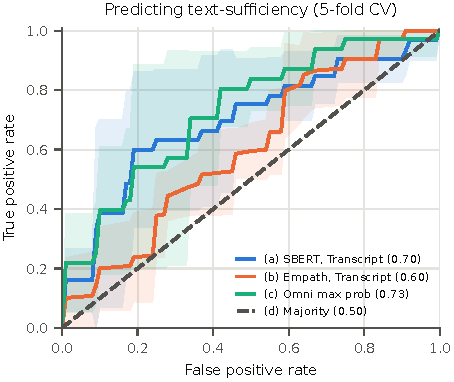
\includegraphics[width=\columnwidth]{figures/predict_roc.pdf}
\caption{Mean ROC curves over five folds (bands: $\pm$1 std) for the best view of each predictor
(model labels). AUROC in parentheses.}
\label{fig:app-roc}
\end{figure}

\begin{figure}[h]
\centering
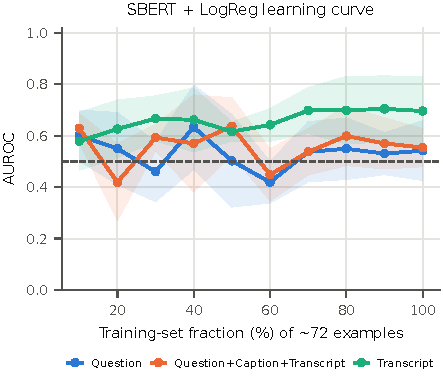
\includegraphics[width=\columnwidth]{figures/predict_learning_curve.pdf}
\caption{Learning curve of SBERT + logistic regression: AUROC on held-out folds when training on a
fraction of each training split (bands: $\pm$1 std over folds; model labels).}
\label{fig:app-lc}
\end{figure}

\paragraph{ROC and learning curves.} In \cref{fig:app-roc}, the model's
confidence and the transcript embeddings perform similarly at low false-positive
rates, and the confidence is better at moderate rates (0.35--0.7); Empath stays
close to chance below a false-positive rate of 0.25. Unlike the transcript
predictor, the confidence needs no training. In \cref{fig:app-lc}, only
the transcript view improves with more data (0.58 at 10\% to 0.70 at 100\%); the
question view stays near chance (0.60 to 0.54) and the combined view does not
improve (0.63 to 0.55). More data might help a transcript-based predictor
somewhat, but it would mostly learn the audio type.

\begin{figure}[h]
\centering
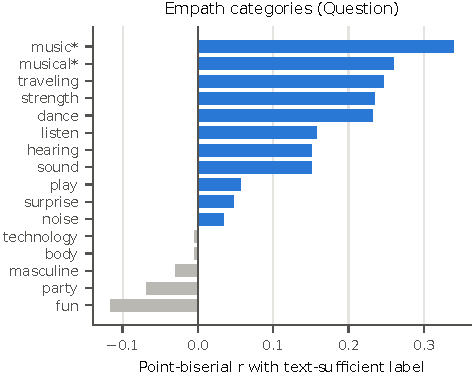
\includegraphics[width=\columnwidth]{figures/empath_top_question.pdf}
\caption{Empath categories in the question text most associated with the model's text-sufficient label
(point-biserial $r$). * marks Benjamini--Hochberg $q<0.05$ over 194 categories.}
\label{fig:app-empath}
\end{figure}

\paragraph{Empath.} \Cref{fig:app-empath} shows the strongest question-view
associations. Only \emph{music} and \emph{musical} survive correction, and the
next categories (\emph{dance}, \emph{listen}, \emph{hearing}, \emph{sound}) are also
audio-related. In the combined view the top categories (\emph{love}, \emph{fire},
\emph{beauty}; $r\approx0.27$--$0.30$) do not survive correction ($q\ge0.35$).
With human labels, nothing survives in any view (smallest $q{=}0.31$). The
interpretable features therefore recover the same signal as the embeddings,
namely the audio type, rather than identifying content that is answerable from
text.
